\cleardoublepage
\setcounter{chapter}{5}
\chapter{\acs{fastPLI}}
\label{chap:Software}
% 
% 
% 
\section{Introduction}\label{sec:fastpliIntro}
%
The previous chapters described the algorithms for creating dense \ac{WM} fiber models (see \cref{chap:sof:modeling}) and for simulating such models in \ac{3D-PLI} (see \cref{cha:sof:simulation}).
Both algorithms are designed to operate autonomously without knowledge of the other.
This can simplify the use of the algorithms for other domains. For example, the fiber models can be used in other in the field of \ac{dMRI} as well (\cite{Ginsburger2019,ginsburgerDis2019}).
However, besides providing algorithms that should be very fast and therefore in this case at a very low level of the programming language (very few abstractions), it is also necessary to provide an API that provides an interface for the user.
This interface must be designed in such a way that the user has a good experience with the algorithms.
Among other things, this means a high level of abstraction with logical and easy-to-use naming systems.
A high level of abstraction in software design means eliminating unnecessary systems and generalizations of functionalities.
\par
%
In addition, the algorithms should be accessible to a wide audience.
Among other things, this means that the program must be installable and easy to understand, even if hardly any programming knowledge is available.
The latter is of course a problem, however, more and more high-level languages have been designed to be easy to understand in the last decades.
\par
%
In summary, this means that a software package must be developed that contains the algorithms and helper functions.
For the above reasons, the \python{} programming language was chosen.
It has become increasingly popular over the last decade, especially in data science.
The core algorithms remain in \cpp{} as described in their chapters to ensure efficiency, speed, and parallelization.
%
\section{fastPLI Toolbox}
%
\begin{figure}[!ht]
\centering
\inputtikz{gfx/fastpli/fastpli_pipeline}
\caption{\acs{fastPLI} package structure.}
\label{fig:fastpli}
\end{figure}
%
The \python{} package is called \acreset{fastPLI} \ac{fastPLI}.
Its source code is publicly available and reviewed in the \ac{JOSS} \cite{fastpli,Matuschke2021}.
The software package includes functionalities for the analysis and visualization of the nerve fiber models as well as for the analysis of the simulation analogous to the current routine experimental measurements, \eg{} inclination analysis.
%
%
%
\subsection{Documentation}
%
\begin{figure}[!t]
    \centering
    \resizebox{\textwidth}{!}{\fbox{
    \begin{tabular}{c|c}
    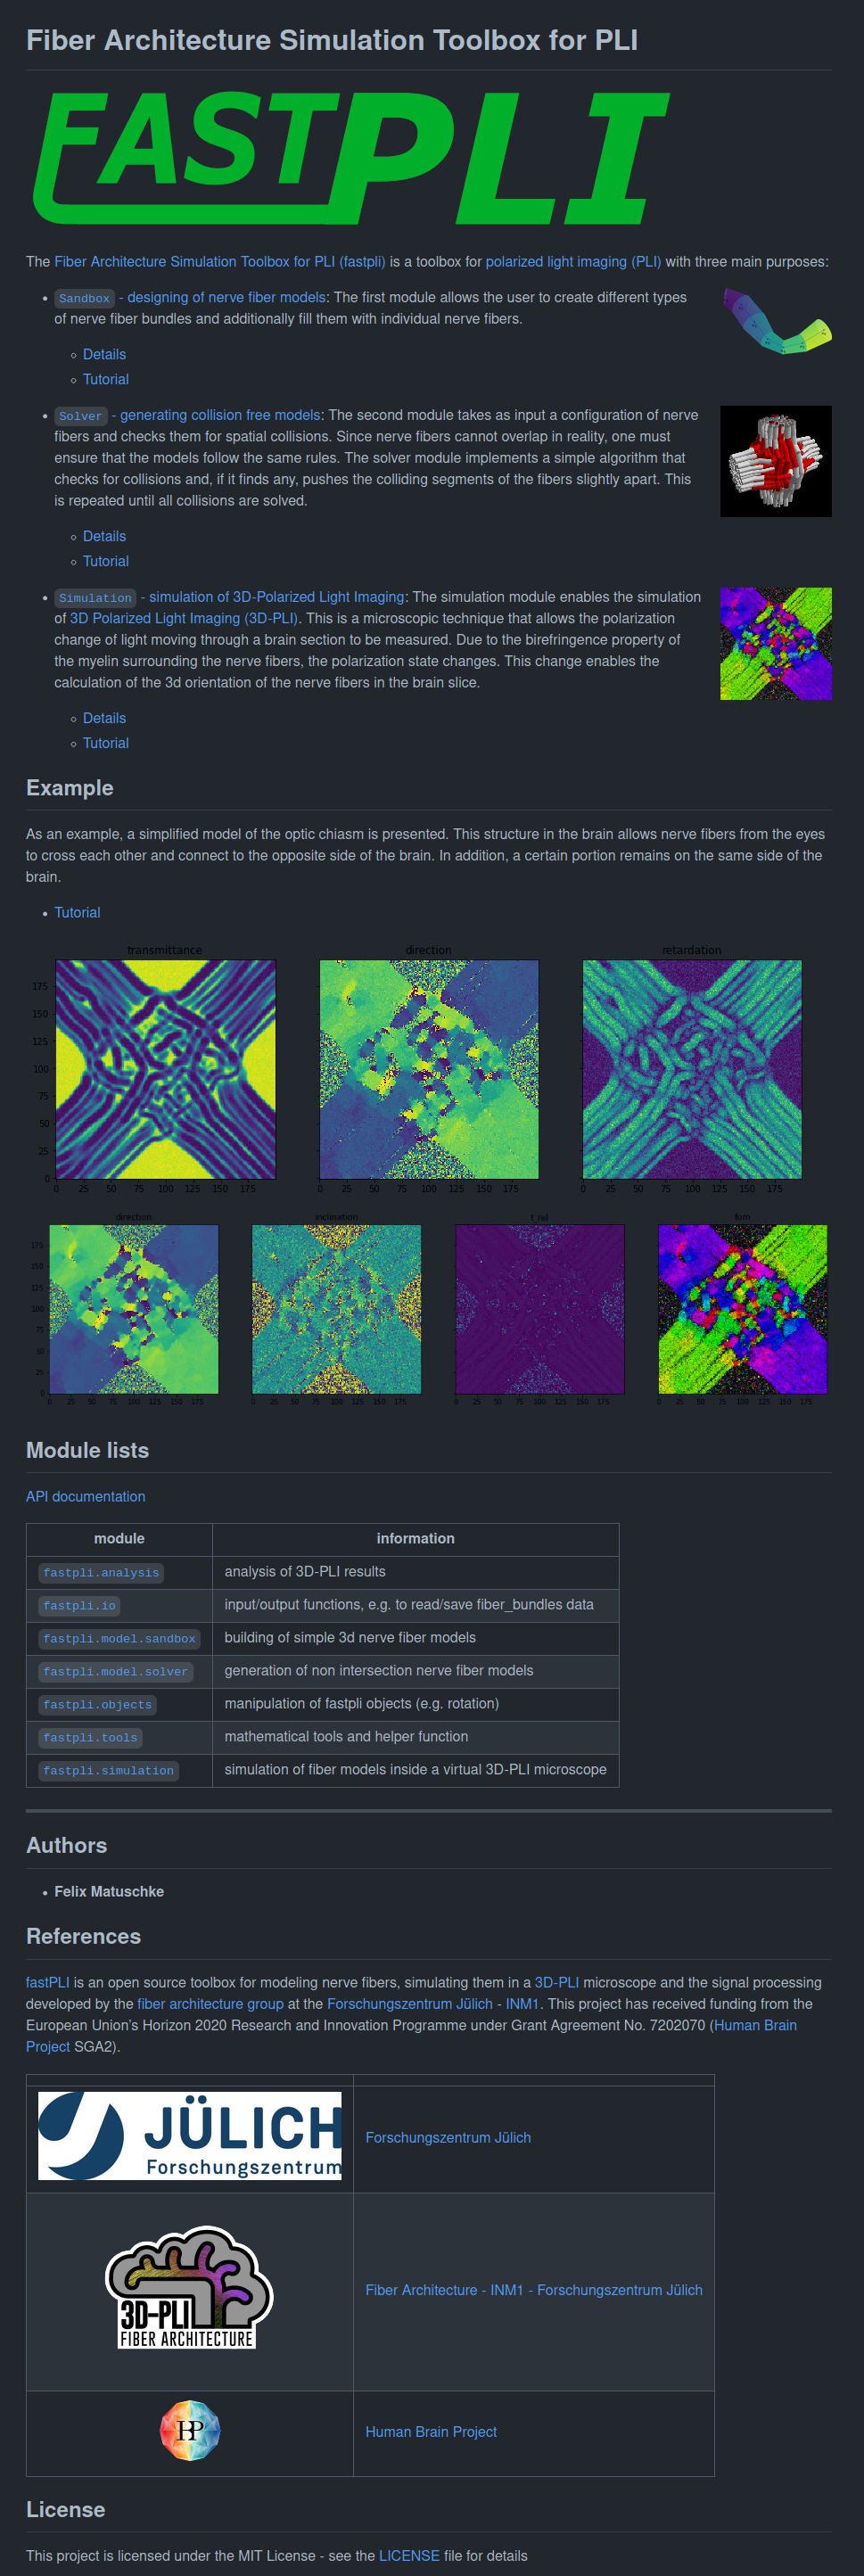
\includegraphics[valign=T,trim=0 1300 0 0, clip]{gfx/fastpli/fastpli_wiki.png} &
 	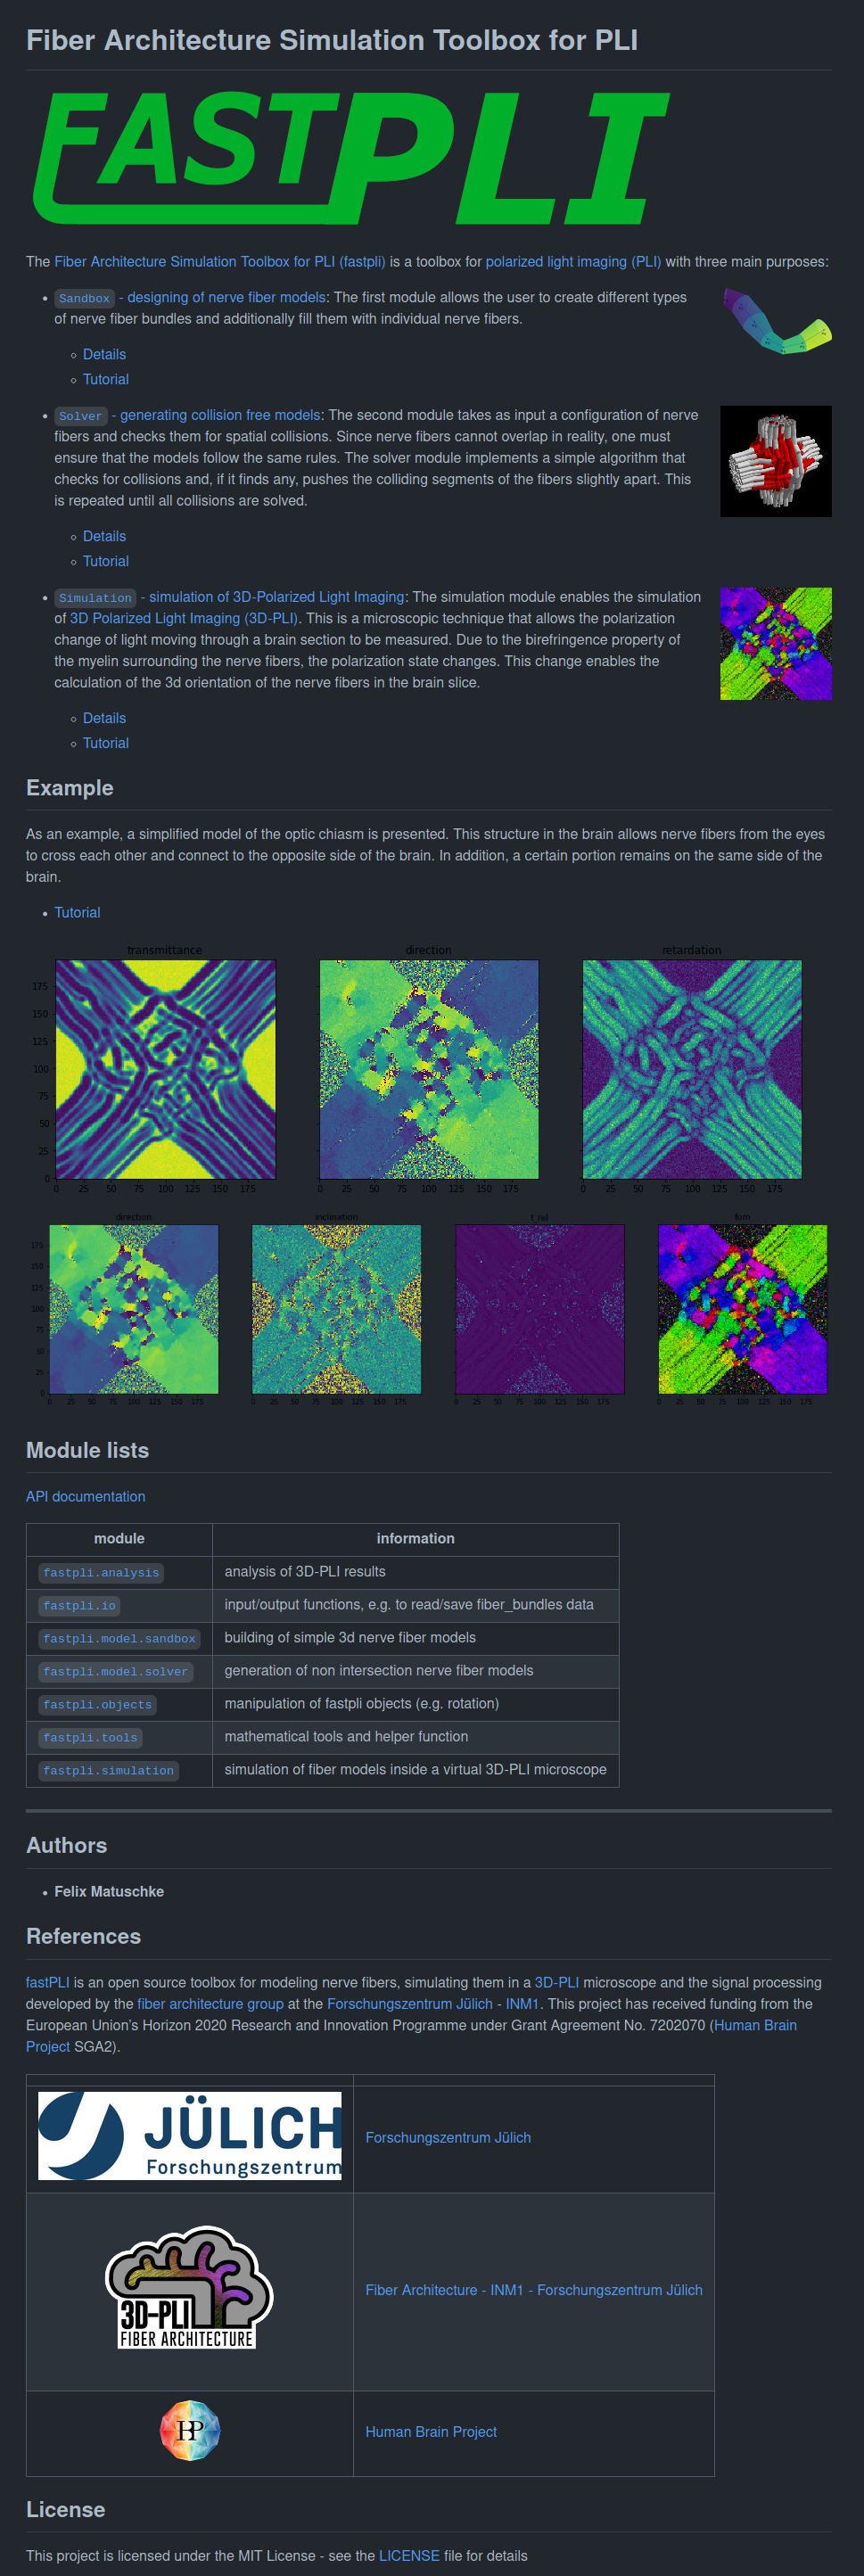
\includegraphics[valign=T,trim=0 0 0 1580, clip]{gfx/fastpli/fastpli_wiki.png} \\
    \end{tabular}
    }}
	\caption{Documentation wiki page of the Github repository \url{https://github.com/3d-pli/fastpli/wiki}.}
	\label{fig:fastpli_wiki}
\end{figure}
%
As is common in software development, all methods are provided with docstrings (documentation strings) so that the user understands their function.
These are, for example, automatically displayed by modern editors during programming to provide assistance.
These docstrings are also used for an automatic release of a \ac{API} documentation.
\footnote{\url{https://3d-pli.github.io/fastpli/}}
In addition to the API, there is a wiki page (see \cref{fig:fastpli_wiki}) that describes the main features, which is an essential part of the review process for release in \ac{JOSS} \cite{Matuschke2021}. 
\footnote{review openly accessible at \url{https://github.com/openjournals/joss-reviews/issues/3042}}
The wiki page is structured like a guide that walks through the aspects of designing nerve fiber models, applying the collision solution algorithm, visualizing nerve fibers, a simple tutorial on \ac{3D-PLI}, and finally applying the models in simulation.
Both executable \python{} scripts and Jupyter notebooks are provided as tutorials to get you started quickly.
For the linking of the individual processes, i.e. generation, simulation and analysis, an example is given of the optic chiasm, the nerve fiber transition of the light pathway from the eyes to the occipital lobe.
%
%
%
\subsection{Dependencies}
%
\paragraph{Python:}
\begin{description}
\item[numpy:] Base N-dimensional array package \cite{2019arXiv190710121V}\\
\url{https://numpy.org/}
\item[scipy:] Fundamental library for scientific computing \cite{2019arXiv190710121V}\\
\url{https://www.scipy.org/}
\item[numba:] Acceleration of Python Functions \cite{Lam2015}\\
\url{https://numba.pydata.org/}
\item[mpi4py:] MPI for Python \cite{Dalcn2005, Dalcn2008, Dalcin2011}\\
\url{https://bitbucket.org/mpi4py/mpi4py/src/master/}
\item[h5py:] HDF5 for Python \cite{collette_python_hdf5_2014, hdf5}\\
\url{https://www.h5py.org/}
\end{description}
%
\paragraph{C++:}
\begin{description}
\item[MPI:] Message Passing Interface \cite{message2015mpi}\\
\url{https://www.mpi-forum.org/}
\item[OpenMP:] Open Multi-Processing, API for multi-platform shared memory multiprocessing programming \cite{dagum1998openmp}\\
\url{https://www.openmp.org/}
\item[OpenGL:] Open Graphics Library \cite{khronos}\\
\url{www.opengl.org}
\item[Pybind11:] Seamless operability between C++11 and Python \cite{pybind11}\\ \url{https://github.com/pybind/pybind11}
\end{description}
%
%
At this point, only Linux builds are supported.
However, for current Windows versions, the \ac{WSL} provides a fully functional Linux kernel within Windows.
This makes it possible to run the same software as on native Linux distributions.
Current macOS versions are not supported, but due to the minimalistic style of the \ac{fastPLI} package, the required changes should be feasible with minimal modifications.
%
%
%
\subsection{Installation}
%
The installation instructions are scripted in a \code{Makefile}.
It first starts a \name{CMake} routine which searches for all the required libraries and programs.
Then the \cpp{} code is compiled and the resulting \name{shared object libraries} are stored in the \python{} routines.
Finally, the provided code \code{setup.py} allows the user to install the compiled package in his environment.
%
\begin{lstfloat}[!ht]
\lstset{style=common}
\begin{lstlisting}
make fastpli
pip3 install .
\end{lstlisting}
\end{lstfloat}
%
%
%
\subsection{Tests, Verification \& Issues}
%
To provide a fully tested software, each module with its main methods is automatically tested with a \name{Github action} after each \name{git push}.
\footnote{github actions are commonly used to automatically build, test, and deploy the software and documentation}.
\footnote{uploud of the current \textit{software stage}.}
This action runs the two latest Ubuntu Long Term Support versions (currently 18.04 LTS and 20.04 LTS) and the most commonly used Python3 versions (currently 3.6 and 3.8) to provide a wide range of supported common versions.
In addition, the \name{Github actions} run all test scripts, check tutorial files, check code format and linting for consistency, and publish the latest documentation after a sucessfull tested release.
\par
%
Github allows to track \name{Issues}.
This feature is originally used to document software bugs.
However, it is also used to discuss ideas, new features, and so on.
As part of the open source release, it was also used communicate with the reviewer.
\footnote{\url{https://github.com/openjournals/joss-reviews/issues/3042}}
This allows to always track back the development process and code changes in addition with the git \name{commits}.
%
% 
% 
\section{Modules}
%
A \python{} \name{package} consists of \name{modules} which contain the definitions of functions, classes and so on.
In the following the different modules are listed alphabetically.
%
%
%
\subsection{\Code{fastpli.analysis}}
%
This module contains all functionalities to analyze the \ac{3D-PLI} simulations analogous to the routine measurements.
This includes the analysis of the signal to the three image modalities transmission, direction and retardation.
Furthermore, it provides the inclination analysis \ac{ROFL} \cite{Schmitz2018}.
In addition, further helper functions exist that provide methods to convert the direction and tilt results into a \ac{FOM}.
\par
% 
For the analysis of fiber models, the module providing a few simple helper functions.
This for example allow the user to generate a histogramm of the orientations of the fiber segments like the ones shown in this thesis.
%
% 
% 
\subsection{\Code{fastpli.io}}
%
This method provides the read and write routines that allow the user to load and save fiber models (\ie{} \code{fiber\_bundles}) to or from disk.
There are two formats available.
The first is a simple text file with the extension \code{.dat} (see \cref{alg:dat-file}).
Here, each $(x,y,z,r)$ tuple of a fiber point is stored as a single line in the file.
Two fibers are separated by one blank line, while two fiber bundles are separated by two blank lines.
This data format is provided to allow a very simple format for manipulating, exchanging and \eg{} reading the files into other programs.
\par
%
\begin{lstfloat}[!ht]
\lstset{style=common,morecomment=[l][\color{syntax_green}]{##},}
\begin{lstlisting}
-6.55 -18.93 -64.98 3.75 # x y z r
-5.73 -14.89 -63.37 3.4
-4.42 -13.66 -58.95 3.05
                         # empty line indicates new fiber
-1.96 -10.07 -52.5 2.92
-1.03 -9.4 -48.62 2.93

                         # two empty lines indicates new fiber bundle
3.4 -4.02 -44.76 3.11
6.22 -1.04 -42.45 3.26
\end{lstlisting}
\caption{Exemplary \name{.dat} file format. Comments are not allowed.}\label{alg:dat-file}
\end{lstfloat}
%
The second format uses \ac{HDF5} \cite{hdf5} which uses a binary data format.
\ac{HDF5} allows the data to be stored as \name{datasets} in \name{groups}.
This is analogous to a file in an operating system being stored in folders.
The \ac{HDF5}-\name{groups} are used to store the \code{fiber} in \code{fiber\_bundle} and \code{fiber\_bundles}.
The $(x,y,z,r)$ information of each fiber is then stored as a 2d-array (see \cref{alg:hdf5}).
%
\begin{lstfloat}[!ht]
\lstset{style=common,morecomment=[l][\color{syntax_green}]{##},}
\begin{lstlisting}
GROUP "/" { # fiber_bundles path
  GROUP "0" { # id of fiber_bundle
      DATASET "0" { # id of fiber
         DATATYPE  H5T_IEEE_F64LE
         DATASPACE  SIMPLE { ( 3, 4 ) / ( 3, 4 ) }
         DATA {
         (0,0): -6.55, -18.93, -64.98, 3.75,
         (1,0): -5.73, -14.89, -63.37, 3.4,
         (2,0): -4.42, -13.66, -58.95, 3.05,
         }
      }
      DATASET "1" { # id of fiber
         DATATYPE  H5T_IEEE_F64LE
         DATASPACE  SIMPLE { ( 2, 4 ) / ( 2, 4 ) }
         DATA {
         (0,0): -1.96, -10.07, -52.5, 2.92,
         (1,0): -1.03, -9.4, -48.62, 2.93,
         }
      }
  }
  GROUP "1" { # id of fiber_bundle
      DATASET "0" { # id of fiber
         DATATYPE  H5T_IEEE_F64LE
         DATASPACE  SIMPLE { ( 2, 4 ) / ( 2, 4 ) }
         DATA {
         (0,0): 3.4, -4.02, -44.76, 3.11,
         (1,0): 6.22, -1.04, -42.45, 3.26,
         }
      }
  }
}
\end{lstlisting}
\caption{Example structure of the fiber format in \ac{HDF5}. This output is generated with the official \code{h5dump} tool.}
\label{alg:hdf5}
\end{lstfloat}
%
%
%
\subsection{\Code{fastpli.model.sandbox}}
%
This module provides all the functions described in \cref{sec:sandbox}.
The module is divided into two submodules: \code{fastpli.sandbox.build} and \code{fastpli.sandbox.seeds}.
\code{fastpli.sandbox.seeds} contains all the methods for populating a 2d-plane, as described in \cref{sec:seeds}.
To populate the fiber from the seeds, the \code{sandbox.build} module provides the methods.
This includes all the described functions from \cref{sec:fillBundle}.
%
%
%
\subsection{\Code{fastpli.model.solver}}
%
The module \code{fastpli.model.solver} contains the compiled solver algorithm, which is explained in detail in \crefrange{sec:Solver}{sec:modelOpt}.
Additionally, the solver algorithm is wrapped in the \code{fastpli.model.solver.Solver} class.
This wrapper class provides a higher level of abstraction (see \cref{sec:fastpliIntro}).
It contains all necessary variables as attributes and therefore provides read/write access via class properties, \eg{} \code{Solver.obj\_mean\_length}.
Each write method checks the input for user errors and returns an appropriate warning or error message.
This class also includes a \code{Solver.get\_dict()} method that returns a \python{} dictionary containing all variables and their values for reproducibility.
It is also possible to store the state of the class with the current state of the \code{fiber\_bundles} as an \ac{HDF5} object.
Finally, this class also provides the possibility to use a simple visualization (see \cref{sec:visualization}) of the solution process.
%
%
%
\subsection{\Code{fastpli.objects}}
%
This module provides a wrapper class for \code{fastpli.objects.fibers} and \code{fastpli.objects.layers}.
Essentially, \code{layers} are a \code{list} of \code{layers}, which in turn are a \code{tuple} of the four attributes \code{absorption}, \code{birefringence}, \code{model}, and \code{scale} (see \cref{sec:dv_generator}).
This wrapper class contains attributes that allow the user to access these values by name, rather than by index \code{tuple} \code{[i]}.
This is helpful to reduce user errors.
\par
% 
The same is true for \code{fastpli.objects.fibers} which contain \code{fastpli.objects.FiberBundles}, \code{fastpli.objects.FiberBundle} and \code{fastpli.objects.Fiber} classes with the same purpose.
\code{FiberBundles} are a \code{list} of \code{FiberBundle} which are a list of \code{Fiber}.
The data of a fiber is stored in a \code{numpy.ndarray} which stores the values contiguously in memory.
Manipulation methods are provided for each class, allowing the user to \code{translate}, \code{rotate}, \code{scale}, and \code{cut} the model.
The latter helps especially in the solution process to reduce the number of objects if only a certain volume is to be generated, since the solution process pushes the fiber objects apart and thus the volume would be increased.
%
%
%
\subsection{\Code{fastpli.simulation}}
% 
Like the \code{fastpli.model.solver.Solver} class, this method provides a wrapper for simulation called \code{fastpli.simulation.Simpli}, which is based on the original algorithm \cite{Dohmen2015,Lucksch2016}.
It contains the two algorithms \code{generator} and \code{simulation} described in \cref{sec:dv_generator,sec:simulation}.
These two algorithms operate separately, but since they share a number of parameters, they coexist within the class.
As in the \code{fastpli.model.solver.Solver} class, all necessary attributes are available and checked for input errors.
Since analysis is usually always performed on the resulting simulations, they are also available in this class and are performed with the same defined parameters as in the simulation.
Methods for saving the variables as \code{dict} or \ac{HDF5} files are also available.
\par
% 
As in the experiment, the simulations can run with the same routine.
This means that many parameters and the simulation pipeline usually do not change.
For this purpose there are \code{pipeline} methods (see \cref{alg:Pipeline}) which provide a high level of abstraction.
Here, all data is automatically analyzed and stored.
%
\begin{lstfloat}[!tb]
\centering
\scalebox{0.75}{
\begin{minipage}{\the\textwidth}
\lstinputlisting[style=python]{code/pipeline.py.tex}
\end{minipage}}
\caption{Simulation pipeline \code{simpli.run\_pipeline()}.}
\label{alg:Pipeline}
\end{lstfloat}
%
%
\subsection{\Code{fastpli.tools}}
% 
The last module contains a set of helper functions.
They provide access to the current version as well as to the git hash so that all calculations can be reproduced.
For fiber modeling, rotation matrices are provided to allow the use of linear algebra.